\documentclass[12pt]{article}
\usepackage{hyperref}
\usepackage{graphicx}
\usepackage{geometry}
\geometry{a4paper, margin=1in}

\title{User Manual Template for Smart Dashboard}
\author{Benjamin Saucedo}
\date{Dec. 10, 2024}

\begin{document}

\maketitle
\tableofcontents
\newpage

\section{Introduction}
Welcome to QTC Smart Dashboard! This dashboard design will be the centralized place to display errors, from various databases, providing a more efficient design instead of having multiple places to go for these errors. This smart dashboard will help consolidate errors, especially in the case of a staff member entering bad data. By seeing the errors easily, service desk staff can assist the people entering bad data to prevent it from happening again in the future. Regarding system errors, they are typically more critical as they may affect the whole infrastructure of an application. Being able to see these errors is necessary for the service desk to communicate with the developers. This Smart Dashboard will help ensuring effective communication and error resolution. Key features include real-time error reporting, error severity rating, and customizable dashboards.

\section{System Requirements}
The software does not interact with any hardware device. Therefore, the software does not require any hardware requirements.

\subsection{Minimum Requirements}
\begin{itemize}
    \item Operating System: Windows with Windows Authentication.
    \item Internet Connection: Required for cloud features.
    \item Web browser with  HTTPS for secure communication.
\end{itemize}

\section{Windows Authentication Installation}
Step-by-step instructions for enabling Windows Authentication.
\begin{enumerate}
    \item Open Control Panel.
    \item Go to Programs and Features.
    \item Select "Turn Windows features on or off"
    \item Expand "Internet Information Services"
    \item Expand "World Wide Web Services"
    \item Expand "Security"
    \item Select the "Windows Authentication" checkbox.
    \item Click OK to confirm
\end{enumerate}

\section{Getting Started}
Guide users through the initial setup and login.
\begin{enumerate}
    \item Launch the software.
    \item Log in using provided credentials or create a new account.
    \item Configure basic settings (e.g., notification preferences).
    \item Explore the interface.
    \item Click on the “?” to access QTC Dashboard Help.(for Dashboard traversal help).
\end{enumerate}

\section{Using the Software}

\subsection{Viewing an Error Report}
\begin{enumerate}
    \item Log in with appropriate credentials.
    \item Navigate to the "Dashboard" section.
    \item Existing errors will be available to view in “Dashboard”.
    \item Click on the “eye” logo to view specified error details.
    \item At the top of the Dashboard, you can make certain selections such as:
        \begin{itemize}
        \item How many errors to show, through drop-down list selection.
        \item Select the type of errors to display by checkbox selection.
        \item Access 200 additional records by selecting “More Pages” button on the bottom right.
	\end{itemize}        
\end{enumerate}

\subsection{Managing Error Reports}
\begin{enumerate}
    \item Access the \textit{Error Management} dashboard.
    \item Filter or sort reports based on criteria (e.g., date, severity).
    \item Assign reports to team members.
    \item Update report statuses (e.g., Open, In Progress, Resolved).
\end{enumerate}

\section{Advanced Features}
Using interfaces, our Smart Dashboard will be able to accept error reports from various databases through Case Management Integration (SQL Server). This allows the user or admin to navigate and access data from the database with the following queue from the dashboard. The queue contains some required fields to allow access and searches.  Users can acquire and manage errors via an API.

\section{Troubleshooting}

\textbf{Problem:} Unable to log in.\\
\textbf{Solution:} Verify credentials and internet connection. Contact support if the issue persists.

\section{FAQs}
Answers to common questions about the software:

\textbf{Q:} Can I customize the error report template?\\
\textbf{A:} Not at this moment but, you can select which type of errors to view through the error display checkbox selection.

\textbf{Q:} How do I navigate the Dashboard?\\
\textbf{A:} By clicking on the “?” to access QTC Dashboard Help, a window will pop up with instructions for common Dashboard navigation instructions.

\section{Contact Support}

\begin{itemize}
    \item Email: \href{mailto:support@example.com}{support@example.com}
    \item Phone: +1-800-555-1234
    \item Chat: Available on our website \href{https://github.com/Armin2708/CS3338-Group4}{link}.
\end{itemize}

\section{Appendices}
QTC: Quality. Timeliness. Customer Service.  
DB: Database
API: Application Programming Interface
LOB: Lines of Business
URL: Uniform Resource Locator

\section{Glossary}
\begin{description}
    \item[QTC] Quality, Timeliness, Customer Service. A term to define key performance metrics.
    \item[API] Application Programming Interface. A set of rules and tools for building software applications.
    \item[DB] Database. A structured set of data held in a computer.
    \item[LOB] Lines of Business. Specific divisions within a company.
    \item[URL] Uniform Resource Locator. The address of a web page.
\end{description}

\section{Figures Section}
\begin{figure}[h]
\caption{Current layout of our Smart Dashboard}
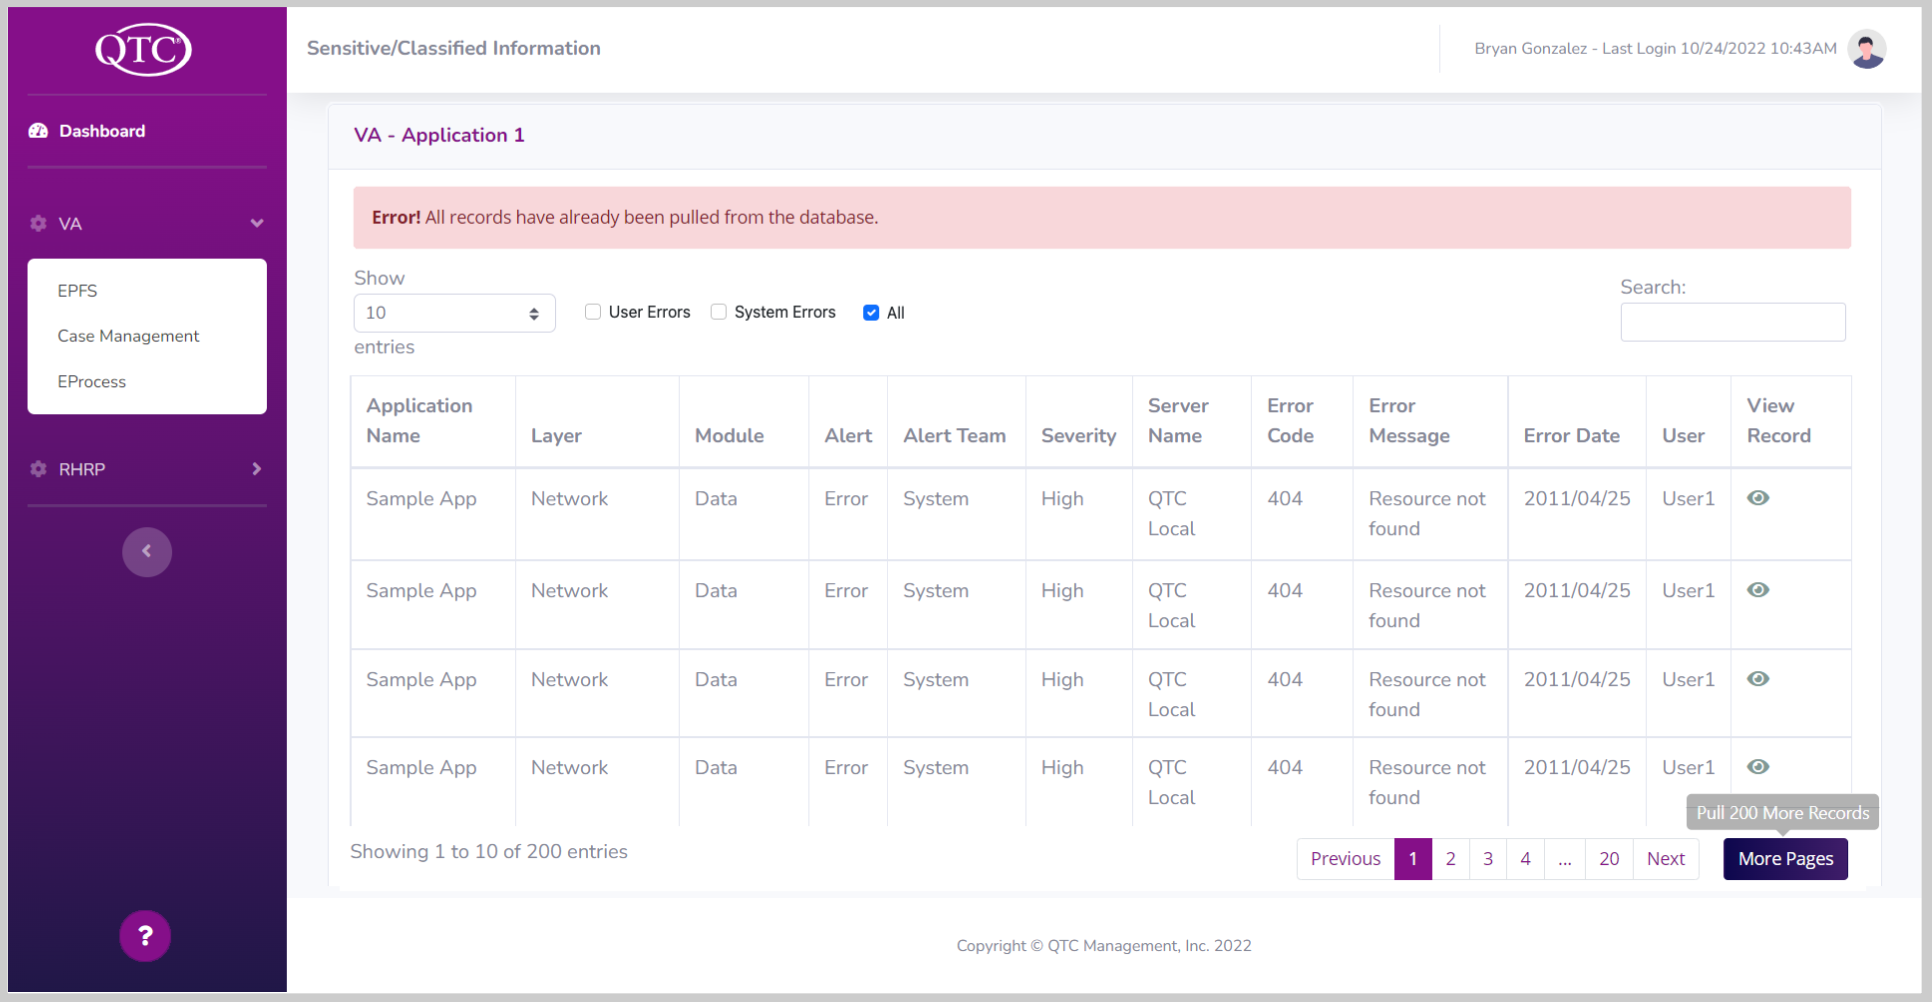
\includegraphics[width=\textwidth]{General}
\end{figure}

\begin{figure}[h]
\caption{Help Window pop out.}
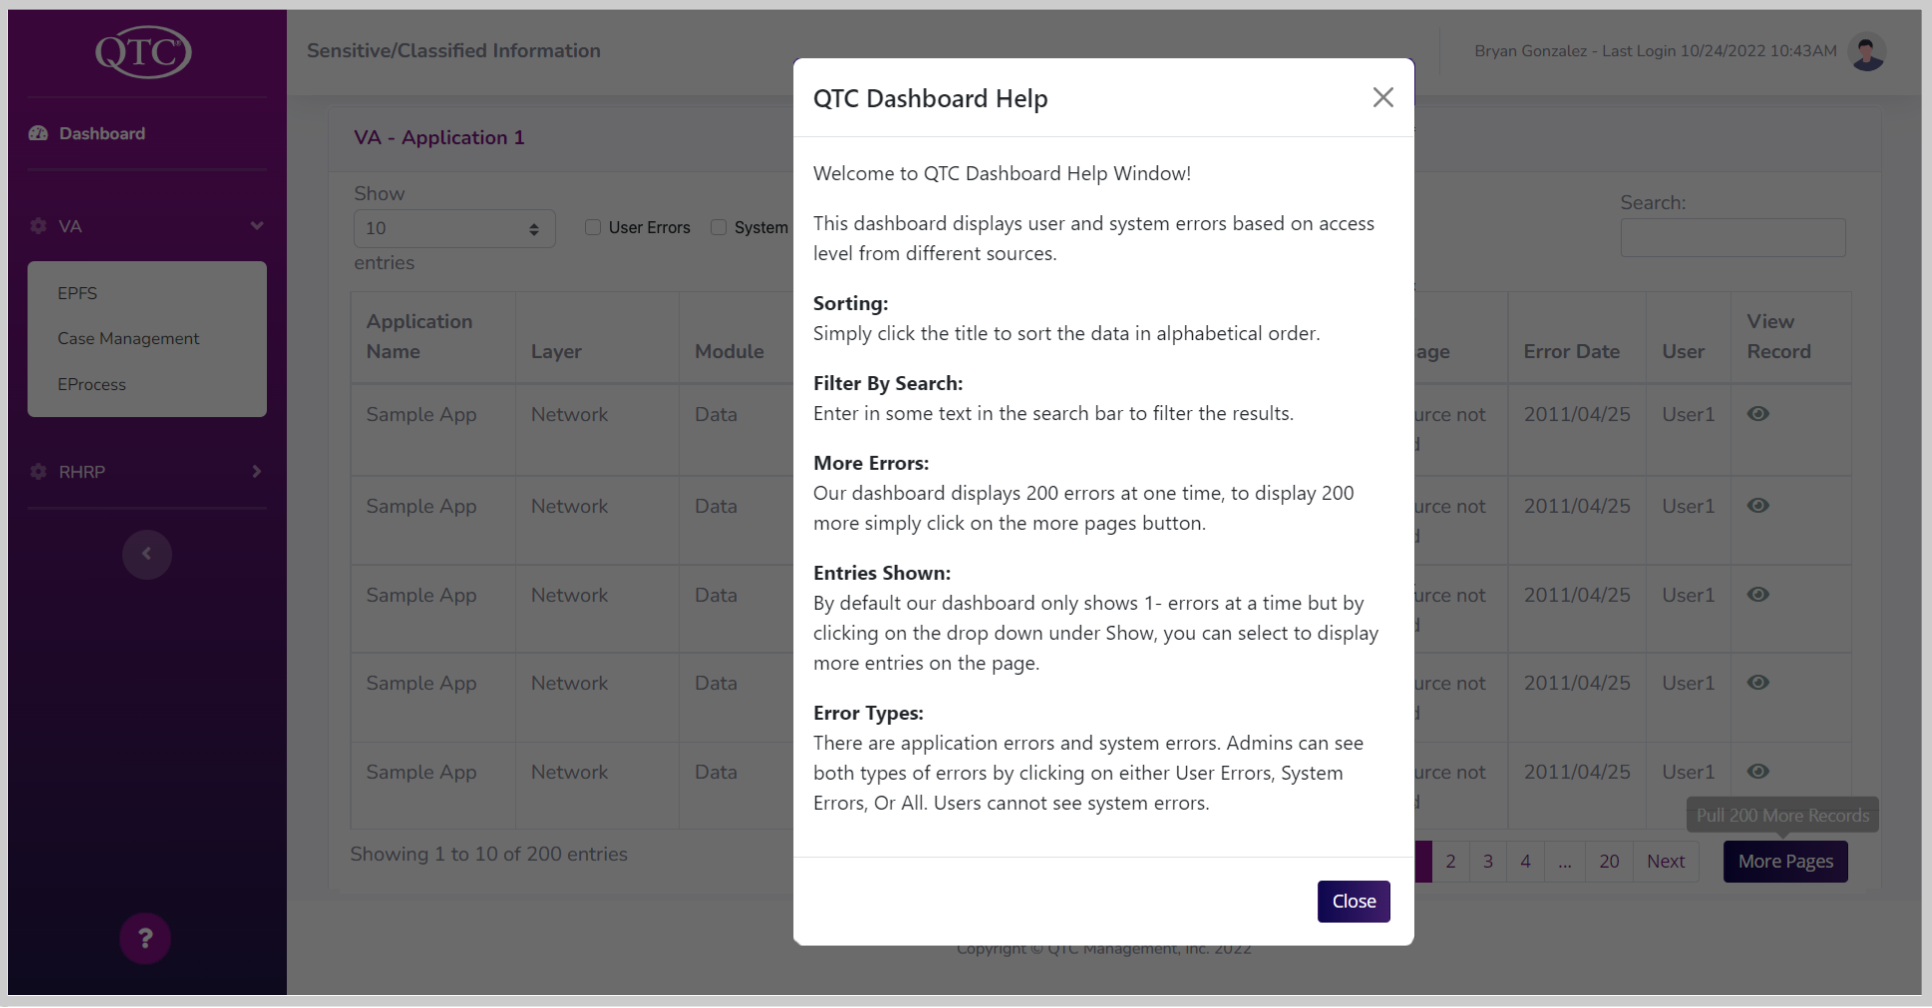
\includegraphics[width=\textwidth]{Help_Window}
\end{figure}

\begin{figure}[h]
\caption{Workflow Diagram}
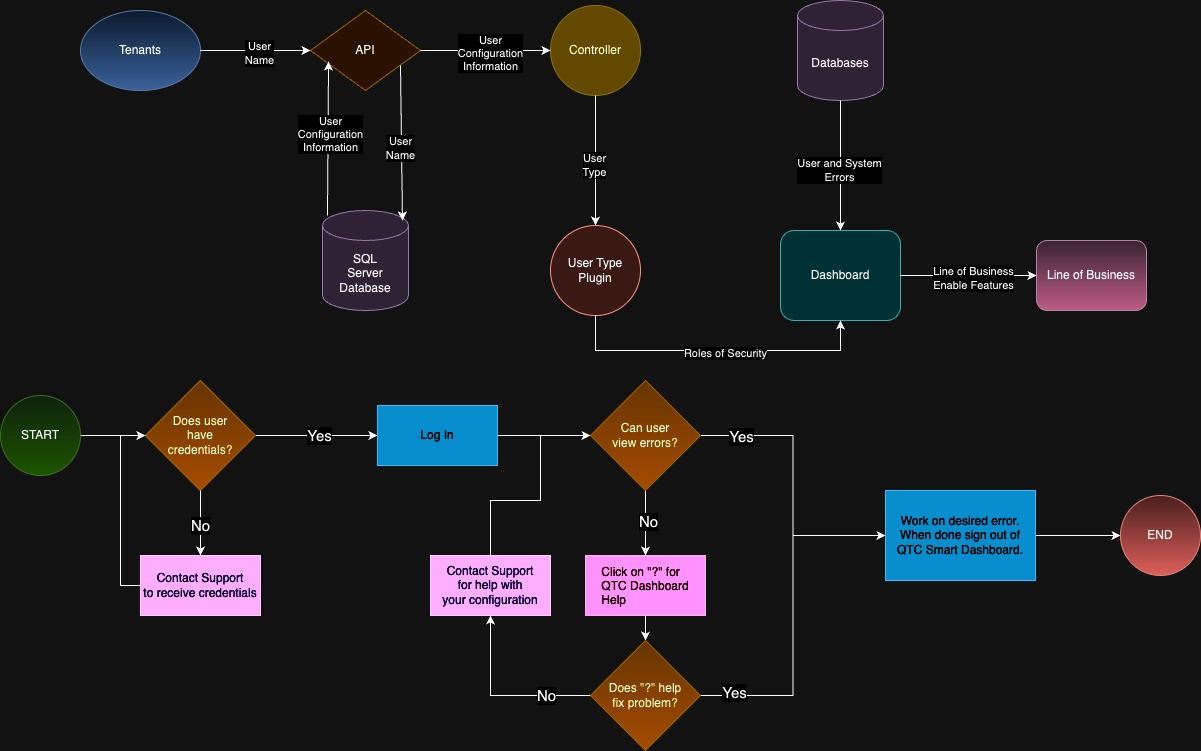
\includegraphics[width=\textwidth]{WorkFlowDiagram}
\end{figure}


\end{document}

